%Linea Para poder completar automaticamente las citas con el Sublime
%No hace el documento, se puede borrar esta linea si no se usa el Sublime
%------------------------------------------------------------------------------
 \newcommand{\NoBiblioMat}[1]{
 \ifthenelse{\equal{#1}{verdadero}}{}{\bibliography{Referencias/base_bibliografica}}
 \NoBiblioMat{verdadero}}
 %-----------------------------------------------------------------------------

%Formato (Nombre de capitulo largo o corto), nombre del capitulo y estilo de la
%Portada del Capitulo
%------------------------------------------------------------------------------

 %Formato en si, titulo en un solo renglon
 \FormatoCapituloUnaLinea

 %Nombre y etiquete para referir
 \chapter{Materiales, Métodos y Procesos}
 \label{chap:Materiales}

 %Para que no salga el numero de pagina en la portada del capitulo
 \thispagestyle{empty}
	
 %Resumen del Capitulo en Italica
  \noindent\textit{En este capitulo se presenta la descripción experimental de todos los procesos involucrados en la tesis. En la primera sección se detallan los procesos de síntesis de las películas mesoporosas, desde la preparación de los soles\index{sol} hasta la caracterización de las mismas; la segunda muestra los procesos de fabricación de los electrodos, desde el diseño a las técnicas de transferencia; la tercera sección describe las técnicas de microscopia\index{microscopía}s utilizadas y la última sección detalla como se llevaron a cabo las mediciones electroquímica\index{electroquimico}s\index{electroquimico}.}


 %Indice de capitulo alineada al borde inferior de la pagina, nueva pagina
 \vfill
 \minitoc
 \newpage

 %-------------------------------------------------------------------------------

\section{Síntesis de películas de sílice mesoporosa}\label{sec:sintesis_mesoporosos}	
	Las consideraciones teóricas sobre la química sol-gel\index{sol-gel} y el autoensamblado inducido por evaporación ya fueron mencionadas en el capitulo \ref{chap:Introduccion}. También fueron mencionadas las razones por las cuales fue elegido el óxido de silicio\index{silicio!oxido de}\index{silicio} y el Pluronic F127\index{Pluronic F127} como estructura para las películas delgadas mesoporosas y como agente moldeante\index{agente moldeante} respectivamente. Los procedimientos, métodos y proporciones molares para la preparación de los soles\index{sol} fueron en su mayoría adaptaciones de los utilizados por Paula Angelomé\index{Angelomé}\cite{Angelome2008} y Cecilia Fuertes\index{Fuertes}\cite{Fuertes2009}. El esquema \ref{esq:peliculas_meso} resume cada etapa de síntesis de las películas, que se explican con detalles en las próximas secciones.
		  \begin{figure}[ht]
			  \begin{center}
			  \includegraphics[width=\textwidth]{Esquemas/Resumen_sintesis_meso.pdf}
			  \caption[Síntesis de películas delgadas mesoporosas]{Diagrama de flujo para la síntesis de películas delgadas mesoporosas.}
			  \label{esq:peliculas_meso}
			  \end{center}
			  \end{figure}

	\subsection{Preparación de los soles}
		La síntesis y depósito\index{depósito} de las películas delgadas mesoporosas de óxido de silicio\index{silicio!oxido de}\index{silicio} (\pdm) comienzan con la preparación de las soluciones, las cuales deben contener los precursor\index{precursor}es del óxido, agente moldeante\index{agente moldeante} de los poros, solvente, H$_2$O y HCl\index{acido@ácido!clohídrico}\cite{Brinker1990}. Cada uno de ellos cumple una función especifica. El precursor\index{precursor} del óxido es el que da la estructura a la película, se utilizó tetraetoxisilano\index{tetraetoxisilano} (TEOS, \textit{Merck}). El surfactante\index{surfactante} es el agente que establece el tamaño de los poros, se utilizó para ello el copolímero de bloque Pluronic F127\index{Pluronic F127} (F127, \textit{Aldrich}) o bromuro de hexadeciltrimetilamonio\index{bromuro de hexadeciltrimetilamonio} (CTAB, \textit{Aldrich}). Como solvente se utilizó etanol\index{etanol} absoluto (EtOH, \textit{Sigma}). El H$_2$O es el reactivo para la formación del óxido, y por último, el HCl\index{acido@ácido!clohídrico} es el encargado de generar el medio ácido\index{acido@ácido} que cataliza la hidrólisis\index{hidrólisis} del TEOS. 
		
		Los reactivos utilizados fueron de calidad proanalisis o superior y el H$_2$O de \SI{18}{\ohm.\cm^{-1}} fue obtenida con un equipo \textit{Ultra Clear TWF} de la marca \textit{Siemmens} (tabla \ref{tabla:reactivos}, pág. \pageref{tabla:reactivos}). 
				\begin{table}[ht]
			  		  \caption[Relación molares de los soles]{Relaciones molares para las soluciones utilizadas.} 
			  		  \begin{tabular}{>{\raggedright\arraybackslash}m{2.2cm}>{\centering\arraybackslash}m{2.2cm}>{\centering\arraybackslash}m{2.2cm}>{\centering\arraybackslash}m{2.2cm}} 
			  		  \toprule
					  Componente & Prehidrolisis  & SiF127  & SiCTAB \\ \midrule
			      	  TEOS 		  & 1			  & 1   	& 1		 \\ \midrule
			      	  EtOH\index{etanol} 		  & 3			  & 40   	& 37	 \\ \midrule
			      	  F127 		  & -		 	  & 0,0075  & -		 \\ \midrule
			      	  CTAB 		  & -             & -		& 0,1	 \\ \midrule
			      	  H$_2$O	  & 1			  & 10   	& 9	     \\ \midrule
			      	  HCl\index{acido@ácido!clohídrico}    	  & 0,00005		  & 0,01   	& 0,01	 \\ 
			      	  \bottomrule
			    	  \end{tabular}
			    	  \label{tabla:soles}
			   		  \end{table}
		Se hizo primero una solución agregando (en este orden) TEOS, EtOH\index{etanol}, HCl\index{acido@ácido!clohídrico} \SI{2,77e-3}{\Molar} y H$_2$O en relaciones molares 1:3:0,00005:1 respectivamente, la cual la llamaremos de ahora en más solución de prehidrólisis. Esta solución se deja envejecer bajo agitación constante durante \SI{48}{\hour}, con el objetivo de hidrolizar el TEOS. 
		Una vez envejecida la prehidrólisis\index{prehidrólisis} se agrega más EtOH\index{etanol}, el surfactante\index{surfactante} y HCl\index{acido@ácido!clohídrico} \SI{2,5e-2}{\Molar}. Los soles\index{sol} obtenidos, que de ahora en más llamaremos SiF127 o SiCTAB, se conservan en \textit{frezeer} a \SI{-18}{\celsius} y solo se saca de allí a la hora de depositarlo. Todos los componentes de las soluciones fueron medidos por pesada en balanza analítica. La tabla \ref{tabla:soles} resume las relaciones molares para cada solución.

		Todas las soluciones fueron preparadas indistintamente en el Centro de Micro y Nanoelectrónica del Bicentenario del Instituto Nacional de Tecnología Industrial (CMNB-INTI) o en la Gerencia Química, Centro Atómico Constituyentes Comisión Nacional de Energía Atómica (CAC-CNEA). 
				\begin{table}[ht] 
						  \caption[Reactivos para los soles]{Nomenclatura, estructura, peso molecular y función de las moléculas utilizadas en las soluciones para la síntesis de películas delgadas mesoporosas de sílice.} 
				  		  \begin{tabular}{>{\raggedright\arraybackslash}m{2.40cm}>{\centering\arraybackslash}m{4cm}>{\centering\arraybackslash}m{2.35cm}>{\raggedright\arraybackslash}m{1.7cm}} 
				  		  \toprule
						  Nombre Nomenclatura    & Estructura & Peso molecular \si{g.mol^{-1}} & Función\\ \midrule
				      	  tetraetoxisilano\index{tetraetoxisilano} TEOS & \includegraphics[scale=0.5]{Esquemas/teos.pdf} & $208,33$ & precursor\index{precursor} del óxido  \\ \midrule
				  		  Pluronic F127\index{Pluronic F127} F127    & \hspace*{-10px} 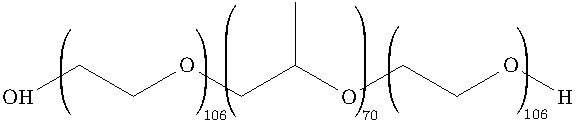
\includegraphics[scale=0.5]{Esquemas/f127.pdf} & \multirow{1}{*}{$13800$}	 & agente moldeante\index{agente moldeante}	 \\ \midrule
				  		  bromuro de hexadeciltrimetilamonio\index{bromuro de hexadeciltrimetilamonio}  CTAB   & \hspace*{1cm} 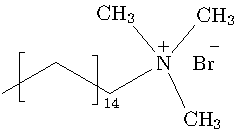
\includegraphics[scale=0.6]{Esquemas/ctab.pdf} & \multirow{1}{*}{$364.48$}	 & agente moldeante\index{agente moldeante}	 \\ \midrule
				  		  ácido\index{acido@ácido} clohídrico\index{acido@ácido!clohídrico} HCl\index{acido@ácido!clohídrico}& \includegraphics[scale=0.75]{Esquemas/hcl.pdf}  & \multirow{1}{*}{$36,46$}   & cataliza la hidrólisis\index{hidrólisis} \\ \midrule
				  		  agua \hspace{2cm} H$_2$O  &  \includegraphics[scale=0.75]{Esquemas/agua.pdf}  & \multirow{1}{*}{$18,02$}   & reactivo de hidrólisis\index{hidrólisis} \\ \midrule
				  		  etanol\index{etanol} \hspace{2cm} EtOH\index{etanol}  & \includegraphics[scale=0.75]{Esquemas/etanol.pdf}  & \multirow{1}{*}{$46,07$}   & solvente \\ 
				  		  \bottomrule
				    	  \end{tabular}
				   		  \label{tabla:reactivos}
				 \end{table}
		
	\subsection{Depósitos de las películas delgadas mesoporosas}\label{sec:deposito_pdm}

			Las películas mesoporosas utilizadas en esta tesis fueron depositadas en el Laboratorio de Fotolitografía del INTI\index{INTI}-CMNB por la técnica de \textit{spin-coating}\index{spin@\textit{spin-coating}}. El equipo utilizado fue un \textit{Suss MicroTec Delta 20BM} el cual consiste en un cabezal rotatorio con control de aceleración de 0 a  \SI{1000}{\min^{-1}.\second^{-1}} y de velocidad variable de 0 a  \SI{10000}{\min^{-1}}; tiene varios portamuestras para sustratos de diferentes tamaños con entrada de vacío para sujetar las muestras (figura \ref{fig:spin}). 
					%figura Spin-coater
					  \begin{figure}[ht]
					  \begin{center}
					  \includegraphics[width=\textwidth]{Imagenes/Spin.jpg}
					  \caption[Equipo para el depósito\index{depósito} de películas delgadas, \textit{spin-coater}]{\textit{Spin-coater} ubicado en el Laboratorio de Fotolitografía del INTI\index{INTI}-CMNB utilizado para el deposito de las películas delgadas mesoporosas, Marca \textit{Suss MicroTec}, modelo \textit{Delta 20BM}.}
					  \label{fig:spin}
					  \end{center}
					  \end{figure}

					   %Rampas
						  \begin{figure}[!ht]
						  \begin{center}
						  \includegraphics[width=0.70\textwidth]{Graficos/rotacion_meso.pdf}
						  \caption[Parámetros de depósito\index{depósito} para las \pdm]{Esquema con las rampas de aceleración, velocidad y tiempo más frecuentes utilizados para el depósito\index{depósito} de \pdm.}
						  \label{fig:rampa-spin}
						  \end{center}
						  \end{figure}
			Se utilizaron como sustrato\index{sustrato} para depositar \pdm , vidrio, silicio, oro\index{oro} sobre silicio, microelectrodo\index{electrodo!microelectrodo}s y sustratos poliméricos como  polimetilmetacrilato (PMMA) y poliestireno de alto impacto (PAI). Cada uno de ellos fue escogido para una función particular (p. ej. sustrato\index{sustrato} para reacciones electroquímica\index{electroquimico}s\index{electroquimico}) o por alguna característica distintiva (p. ej. transparente en el IR), el detalle se describe en la tabla \ref{tabla:sustratos}, pág. \pageref{tabla:sustratos}.
			Las dimensiones de de las muestras fueron de \SI{1x1}{\cm} a \SI{2x2}{\cm} en la mayoría de los casos, aunque se utilizaron más grandes y hasta obleas completas de \SI{10}{\cm} de diámetro. Antes del depósito\index{depósito} se filtra el sol\index{sol} con un filtro de jeringa\index{jeringa} de \SI{0.45}{\um}. Para realizar el deposito se utilizaron pipetas Pasteur o pipetas automáticas dependiendo del volumen requerido que varió de 80 a \SI{100}{\uL.\cm^{-2}}. Las condiciones del laboratorio durante el depósito\index{depósito} se mantuvieron en \SI{25}{\celsius} y entre 30\% y 50\% de HR.					  
			Inmediatamente luego de colocar el sol\index{sol} sobre el sustrato\index{sustrato} se dió comienzo a la rotación. La evaporación del solvente promueve la formación del cristal líquido\index{cristal líquido} por el mecanismo de autoensamblado molecular\index{autoensamblado molecular} inducido por evaporación, mecanismo explicó oportunamente en el capitulo \ref{chap:Introduccion}, pág. \pageref{sec:mesoporosos}. El espesor del depósito\index{depósito} ($t$) es inversamente proporcional a la raíz cuadrada de la velocidad angular\index{velocidad!angular} ($\omega$)\cite{Meyerhofer1978,Hall1998} (ec. \ref{eq:spin}), por lo que las rampas de velocidad y aceleración utilizadas fueron optimizadas para lograr espesores entre 150 y \SI{300}{\nm}\cite{Nano-compuestas2013}. 
					\begin{equation}
			 		    t\propto \frac{1}{\sqrt{\omega}}
			 		     \label{eq:spin}
						\end{equation}
			Los esquemas aplicados están plasmados en la figura \ref{fig:rampa-spin}.
		 	      \begin{table}[ht]
		  		  \caption[Sustratos utilizados para el depósito\index{depósito} de \pdm]{Sustratos utilizados para el depósito\index{depósito} de \pdm.} 
		  		  \begin{tabular}{>{\raggedright\arraybackslash}m{2.4cm}>{\raggedright\arraybackslash}m{2.5cm}>{\raggedright\arraybackslash}m{2cm}>{\raggedright\arraybackslash}m{3.55cm}} 
		  		  \toprule
				  Sustrato Nomenclatura   & Observaciones  & Limpieza previa$^*$ & Función \\ \midrule
		       	  vidrio\index{vidrio} \hspace{2cm} Vi  &	portaobjetos \textit{BioTraza} & inmersión KOH 40\% & económico para pruebas preliminares de deposito \\ \midrule
		       	  silicio\hspace{2cm} Si  & Si[100] pulido dopado tipo n  \textit{Addison}& inmersión HF\index{acido@ácido!fluohídrico} 48\% & FTIR,SEM\index{SEM},FIB\index{FIB}, EPA \\ \midrule
		       	  Au\index{oro} sobre silicio\hspace{2cm} Si$|$Au & depositado por pulverizacion catódica$^\dagger$  & ultrasonido\index{ultrasonido}en H$_2$O  & transporte, EQ\\ \midrule
		      	  microelectrodo\index{electrodo!microelectrodo}s \hspace{2cm} $\mu Elec$ & sensores, diseño transferido por fotolitografía\index{fotolitografía}$^\mathsection$  	  &  ultrasonido\index{ultrasonido}en H$_2$O  & multisensado, EQ \\ \midrule
		      	  polimericos         &  PMMA y PAI		  &  ultrasonido\index{ultrasonido}en H$_2$O &  demostrador métodos suaves de síntesis\\ 
		      	  \bottomrule
		    	  \end{tabular}\vspace*{2pt}
		    	  \footnotesize{$^*$Ver la sección <<\nameref{sec:limpieza}>>, tabla \ref{tabla:limpieza}, pág. \pageref{sec:limpieza}.}\\
		    	  \footnotesize{$^\dagger$Ver la sección <<\nameref{sec:sputt}>>, pág.\pageref{sec:sputt}.} \\
		    	  \footnotesize{$^\mathsection$Ver la sección <<\nameref{sec:fotolito}>>, pág. \pageref{sec:sputt}.}
		    	  \label{tabla:sustratos}
		   		  \end{table}
			
				  \pagebreak

	\subsection{Condensación y extracción\index{extracción}}\label{sec:cond_y_extr}

		Una vez realizado el depósito, se debe conservar la estructura del cristal líquido\index{cristal líquido} obtenido, y evitar el deterioro durante la eliminación del surfactante\index{surfactante}, para ello se estabiliza la película durante 1 hora en cámara de humedad controlada a 50\% de HR. Para mantener la humedad constante en 50\% de HR se utilizó una solución satura de de Ca(NO$_3$)$_2$.5H$_2$O (\textit{Biopack}). El ingreso de H$_2$O permite de esta forma aumentar el grado de polimerización del óxido y ayudar a la separación de fases entre el agente moldeante\index{agente moldeante} y el óxido. El proceso de estabilización y condensación\index{condensación} del óxido continua con un calentamiento en plancha calefactora, (\textit{Cimarec}) una hora a \SI{60}{\celsius} y una hora más a \SI{130}{\celsius}\cite{Crepaldi2003,Crepaldi2002a}. 
			\begin{figure}[ht!]
						  \begin{center}
						  \includegraphics[width=\textwidth]{Esquemas/Resumen_extraccion.pdf}
						  \caption[Tratamientos post-síntesis de \pdm]{Etapas de estabilización y diferentes tratamientos post-síntesis utilizados para hacer las \pdm.}
						  \label{esq:peliculas_meso_tratamientos}
						  \end{center}
						  \end{figure}
		Posteriormente a la estabilización de la película se experimentaron varios tratamientos para completar el proceso de condensación\index{condensación} y extraer el surfactante\index{surfactante} para dar lugar a la película nanoporosa, a saber:

				\begin{itemize}

				\item \textit{Calcinacion.} Este es el proceso clásico en el cual se somete a la película a una temperatura de \SI{350}{\celsius} durante \SI{2}{\hour} con una rampa de \SI{1}{\celsius.\min^{-1}} (Horno \textit{Indef 337}). De esta forma se condensa el óxido, se elimina el surfactante\index{surfactante} y se minimiza el daño de la estructura tridimensional de la red nanoporosa\index{película!nanoporosa} \cite{Crepaldi2003}.

				\item \textit{Condensación ácida.} En este método se busca promover la condensación\index{condensación} de la matriz inorgánica mediante la exposición de las películas a una atmósfera de vapores de HCl\index{acido@ácido!clohídrico} \cite{Doshi2000a}. El arreglo para tal fin consiste en sujetar las muestras al fondo de un vaso precipitado y ponerlo boca abajo sobre un cristalizador con HCl\index{acido@ácido!clohídrico} concentrado (\textit{Biopack}) durante \SI{10}{\min}. 

				\item \textit{Condensación básica.} Al\index{aluminio} igual que el método anterior, se busca promover la condensación\index{condensación} del óxido cambiando las condiciones del entorno químico, en este caso someter las películas a una atmósfera de pH\index{pH} extremadamente básico\index{básico} generada con vapores de NH\index{amoniaco}$_3$ (\textit{Biopack}) \cite{Soler-Illia2012,Soler-Illia2011}. El armado experimental fue igual que el descripto para el método ácido.

				\item \textit{Prolongado a 130.} Esta estrategia de síntesis involucró dejar las muestras en estufa a \SI{350}{\celsius} durante 7 días con el objetivo de promover la condensación\index{condensación} del óxido.

				\item \textit{Alto vacío.} El último experimento que se estudió fue  el de dejar las muestras en una cámara de alto vacio\index{alto@alto vacío} \SI{1e-5}{\milli\bar} a \SI{130}{\celsius} durante 7 días. Para calentar y lograr el vacío necesario se utilizó la cámara de una soldadura de obleas (\textit{EVG 501 Manual Wafer Bonding System}) la cual fue evacuada por una bomba mecánica y una turbomolecular secuencialmente.

				\end{itemize}
					
		En los casos donde fue necesario realizar la extracción\index{extracción} del surfactante\index{surfactante} (no calcinando) se realizó colocando las muestras en un reflujo de isopropanol\index{propanol@2-propanol} a punto de ebullición (\textit{Biopack}) durante \SI{15}{\min}, luego de esto se realiza un enjuague con H$_2$O acidificada con HCl\index{acido@ácido!clohídrico}, pH\index{pH}$\approx$2.
			  
	\subsection{Espectroscopia IR}\label{sec:IR}

		El segmento infrarrojo (IR) del espectro electromagnético puede ser divido en tres zonas, según su longitud de onda\index{longitud de onda}, IR cercano (400 a \SI{10}{\cm^{-1}}), IR medio (4000 a \SI{400}{\cm^{-1}}), e IR lejano (14000 a \SI{4000}{\cm^{-1}}). El infrarrojo medio puede ser usado para estudiar las vibraciones\index{vibración} fundamentales y la estructura roto-vibracional; brinda información acerca de los grupos orgánicos e inorgánicos  presentes a través del análisis de las vibraciones\index{vibración} moleculares.\cite{Atkins2006,Barrow1962,Stuart2004} 
		
		A lo largo de este trabajo se uso esta porción del espectro IR para analizar los resultados de la extracción\index{extracción} de surfactante\index{surfactante} y estructura inorgánica de las \pdm. Las mediciones se llevaron a cabo en la Unidad Técnica de Nanomateriales del Centro de Investigaciones en Procesos Superficiales del INTI\index{INTI} (INTI-CIEPS). El equipo es un \textit{Thermo Scientific Nicolet 6700 FTIR} que cuenta con un microscopio para poder focalizar el haz en un área de aproximadamente \SI{0.5x0.5}{\mm}. Se utilizó la técnica de espectroscopia\index{espectroscopia} infrarroja por transformadas de Fourier (FTIR) tanto en trasmisión como en reflexión y los espectros fueron tomados con el detector MCT/B (\textit{Wide Band mercury/cadmiun/telluride}) que es de 4 a 10 veces más sensible que los detectores estándar para equipos de espectroscopia\index{espectroscopia} FTIR.\cite{Nicholet2007} Las películas destinada a ser caracterizadas por FTIR\index{FTIR} fueron depositadas sobre Si, por ser este trasparente en el IR medio.

	\subsection{Ángulo de contacto}

		Las medidas de ángulo de contacto\index{angulo@ángulo de contacto} se realizaron en la Gerencia Química, CAC-CNEA con un equipo \textit{Ramé-Hart 290} y los datos fueron recogido con el software \textit{DROPImage} que brinda herramientas de análisis para calcular el ángulo de contacto\index{angulo@ángulo de contacto}. Estas medidas se utilizaron principalmente como parámetro de entrada para calcular, mediante la técnica de elipsoporosimetría, la distribución de los tamaños de poro\index{poro} y cuello\index{cuello de poro} de los sistemas estudiados.\cite{Boissiere2005}

	\subsection{Elipsometría}\label{sec:elipso}

		La elipsometría es una técnica de análisis óptico que se basa en el cambio del estado de polarización de la luz que incide sobre una o más películas delgadas soportadas sobre un material reflectivo. Dicho análisis es no destructivo y es útil para la determinación de espesores y constantes ópticas (índices de refracción y constante de absorción) de dichas películas.\cite{TompkinsHarlandG.1999,Rothen1945} Las mediciones obtenidas nos devuelven los parámetros elipsométricos $\Delta$ y $\Psi$. 

		Mediante un modelo matemático (en el cual se proponen valores iniciales para las constantes ópticas y el espesor de la muestra) se ajusta por cuadrados mínimos hasta minimizar, por sucesivas iteraciones, la diferencia con los datos experimentales y de esta forma obtenemos el espesor y el índice de refracción\index{indice@índice de refracción} de la película. Cuando se adapta una cámara al equipo, donde se puede variar la presión parcial de H$_2$O, se pueden medir los cambio de las propiedades ópticas de películas delgadas porosas durante la adsorción\index{adsorción} y desorción\index{desorción} de H$_2$O. A esta técnica se la conoce con el nombre de porosimetría elipsométrica ambiental o elipsoporosimetría ambiental (EPA). La figura \ref{fig:elipso} esquematiza el funcionamiento del elipsómetro y la figura \ref{fig:elipsofoto}, pág \pageref{fig:elipsofoto}, es una fotografía del instrumental que se utilizó. Se construye de esta forma una isoterma\index{isoterma} de adsorción\index{adsorción}/desorción 
			  \begin{figure}[t]
			  \begin{center}
			  \includegraphics[width=\textwidth]{Esquemas/Elipso.pdf}
			  \caption[Esquema de la técncia de elipsoporosimetría ambiental]{Esquema de los componentes principales del equipos de elipsometría utilizado para determinar las constantes elipsométricas, $\Delta$ y $\Psi$, de las cuales se obtienen el espesor, indice de refracción, coeficiente de absorción,  distribución y tamaño de poro\index{distribución!de poro}s y cuello\index{cuello de poro}s de las \pdm.}
			  \label{fig:elipso}
			  \end{center}
			  \end{figure}
		de H$_2$O en función del índice de refracción\index{indice@índice de refracción} de la/s películas porosas.\cite{Baklanov2000,Boissiere2005,Sing1985} El volumen de vapor adsorbido dentro de los poros se determina luego a partir de dicha variación utilizando aproximaciones de medio efectivo como la de Bruggeman\index{Bruggeman}\cite{Bruggeman1935} o la de Maxwell-Garnett\index{Maxwell-Garnett}\cite{Garnett1906} que son simplificaciones de la ecuación general de Lorentz-Lorentz\index{Lorentz-Lorentz} \cite{TompkinsHarlandG.1999}.
		La aproximacion de Bruggeman\index{Bruggeman} considera dos componentes mezclados al azar cuyas fracciones en volumen ($f_i$) y constante dielectrica ($\mathcal{E}_i$) deben cumplir con la ecuación \ref{eq:bruggeman} donde $\mathcal{E}_e$ es la constante dieléctrica del material compuesto, la cual se determina experimentalmente.
								\begin{equation}
					 		   	 f_1\left(\frac{\mathcal{E}_1-\mathcal{E}_e}{\mathcal{E}_1+2\mathcal{E}_e}\right)+
					 		   	 f_2\left(\frac{\mathcal{E}_2-\mathcal{E}_e}{\mathcal{E}_2+2\mathcal{E}_e}\right)=0
					 		     \label{eq:bruggeman}
								\end{equation}
		La aproximación de Maxwell-Garnett\index{Maxwell-Garnett} considera al material compuesto por al menos dos especies, la matriz y la inclusión. En el caso de los óxidos porosos, la matriz es el óxido y el aire el surfactante\index{surfactante} la inclusión. Se deben satisfacer en este caso las ecuaciones \ref{eq:maxwall1} y \ref{eq:maxwall2}.
							\begin{equation}
					 		   	 f_1\left(\frac{\mathcal{E}_1-\mathcal{E}_2}{\mathcal{E}_1+1\mathcal{E}_2}\right)-
					 		   	 \left(\frac{\mathcal{E}_e-\mathcal{E}_2}{\mathcal{E}_e+2\mathcal{E}_2}\right)=0
					 		     \label{eq:maxwall1}
								\end{equation}
								\begin{equation}
					 		   	 f_2\left(\frac{\mathcal{E}_2-\mathcal{E}_1}{\mathcal{E}_1+2\mathcal{E}_1}\right)-
					 		   	 \left(\frac{\mathcal{E}_e-\mathcal{E}_1}{\mathcal{E}_e+2\mathcal{E}_1}\right)=0
					 		     \label{eq:maxwall2}
								\end{equation}
		El volumen total ocupado por los poros, V$_p$, y el volumen de agua adsorbido para cada HR, V$_{ads}$, se calcularon aplicando indistintamente dichas aproximaciones (ya que para \pdm\space dan resultados equivalentes) a las constantes dieléctricas medidas del film seco y lleno de agua, luego de la condensación\index{condensación} capilar.\cite{Angelome2008,Fuertes2009,Nano-compuestas2013}
		El tamaño de los poros y los cuello\index{cuello de poro}s, que forman la red porosa tridimencional, se puede calcular a partir de la rama de adsorción\index{adsorción} y de la de desorción\index{desorción} de la isoterma\index{isoterma} respectivamente. Para ello debemos recurrir a la ecuación de Kelvin\index{Kelvin} (ec. \ref{eq:kelvin}), que describe el equilibrio líquido-vapor considerando tamaño de la esfera y energía\index{energía} superficial. Donde R es la constante de los gases, T es la temperatura, P es la presión de vapor\index{presión de vapor}, P$_s$ es la presión de vapor\index{presión de vapor} de saturación, $\gamma$ es la tensión superficial\index{tensión superficial} del líquido, V$_m$ es el volumen molar del líquido y $\theta$ es el ángulo de contacto\index{angulo@ángulo de contacto} sólido-líquido. 
								\begin{equation}
					 		   	 \ln \left(\frac{P}{P_s}\right)=\frac{2\gamma V_m}{RT} \cos{\theta}\frac{\partial S}{\partial V}
					 		     \label{eq:kelvin}
								\end{equation}			
		Para poros esféricos la relación $\partial S/ \partial dV$ es proporcional al radio de la esfera, llamado radio de Kelvin\index{Kelvin}.\cite{FernandezPrini2005}

		Las medidas fueron tomadas en la Gerencia Química, CAC-CNEA con un  elipsómetro espectroscópico marca \textit{SOPRA}, modelo \textit{GES 5E}. El equipo cuenta con una lámpara cuyo rango espectral es de 190 a \SI{900}{\nm}, pose una cámara para realizar las mediciones en condiciones de humedad controladas y también permite configuración en modo \textit{micro-spot} que permite reducir el área de medición a una región de aproximadamente \SI{1}{\mm^2}. El modelado de los parámetros se hizo mediante el \textit{software Winelli II} también de la marca \textit{SOPRA}.
					\begin{figure}[h]
							  \begin{center}
							  \includegraphics[width=\textwidth]{Imagenes/elipsometro.jpg}
							  \caption[Elipsómetro]{Foto del equipos elipsómetro espectroscópico marca \textit{SOPRA}, modelo \textit{GES 5E} ubicado en la Gerencia Química, CAC-CNEA utilizado para la caracterización de las \pdm.}
							  \label{fig:elipsofoto}
							  \end{center}
							  \end{figure}

\section{Microfabricación de los electrodos}
		
	En esta sección se dará cuenta de los detalles experimentales para la fabricación de los electrodos, los cuales son una parte fundamental de los sensores. Es en la superficie\index{superficie} de los electrodos donde ocurren la reacciones oxido-reducción de los analitos de interés (es decir, el intercambio de electrones entre moléculas que queremos detectar y el electrodo) y es allí donde se deposita la película delgada \index{película!delgada}mesoporosa. Es por ello que es fundamental contar con un diseño funcional y compacto y, además, controlar los aspectos superficiales tales como la rugosidad\index{rugosidad}, control de impurezas, espesor, y funcionalización de ser necesario. 

	Los electrodos fueron enteramente diseñados y fabricados en los laboratorios del CMNB-INTI. 
		
	Las herramientas y técnicas utilizadas para la fabricación son propias el sector de la microelectrónica\index{microelectrónica}; herramientas de \textit{software}\index{software@\textit{software}} tipo CAD, fotolitografía\index{fotolitografía}, pulverización catódica\index{pulverización catódica}, grabado por vía húmeda, \textit{lift-off}\index{lift@\textit{lift-off}}, corte y encapsulado, etc.\cite{Franssila2004,Jaeger2001} Cada uno de estos procesos se explicará en las secciones subsiguientes. 

	El esquema general de trabajo para la transferencias de una o más capas se presenta en la figura \ref{esq:micro}.

			\begin{figure}[ht]
			  \begin{center}
			  \includegraphics[width=\textwidth]{Esquemas/Resumen_micro.pdf}
			  \caption[Esquema para la transferencia de los diseños\index{transferencia!de los diseños}\index{transferencia!de los diseños}]{Diagrama general para la transferencias y fabricaciones de diseños de una o más capas. Este esquema contempla el uso de las técnicas de \textit{lift-off }o grabado según se requiera dependiendo de las características de los materiales empleados para esa capa.}
			  \label{esq:micro}
			  \end{center}
			  \end{figure}
			  
	\subsection{Diseño e impresión de las máscara\index{máscara}s}\label{sec:impresion_mascaras}

		El primer paso necesario en la fabricación de los sensores\index{sensor} es el diseño. Como todo diseño en microelectónica, se pensó en función de la tecnología disponible, de la calidad de las máscara\index{máscara}s y de la aplicación final. Todos estos aspectos ya fueron expuestos en el capitulo \ref{chap:Introduccion}, por lo que aquí nos remitiremos a establecer los detalles técnicos.

		Los diseño se pensaron para obleas de \SI{10}{\cm} de diámetro. El primer diseño se mandó a imprimir en filmina de \SI{13x13}{\cm} en una filmadora de películas \textit{Agfa Accuset 1000} de la firma $Imacrom$ a una resolución de \SI{3600}{dpi}, lo que permitió obtener resoluciones de linea de \SI{50}{\um}, muy por encima de la resolución de la tecnología de la cual disponemos (transferencia por UV, $\lambda=365nm$). El segundo diseño, mas completo e integrado, tambíen se pensó para obleas \SI{10}{\cm} de diámetro. Este contempló la integración del contraelectrodo\index{electrodo!contraelectrodo} y el electrodo de referencia\index{electrodo!de referencia}, además de incluir 6 electrodos de trabajo\index{electrodo!de trabajo}. Las máscara\index{máscara}s correspondientes a este diseños se mandaron a imprimir en filminas de \SI{13x13}{\cm} a la empresa \textit{International Phototool Company} en una resolución de \SI{48000}{dpi}, logrando mejor resolución y lineas más definidas que en el primer diseño, hasta de \SI{7}{\um}. Todos los diseños se llevaron a cabo con el \textit{software CAD electric}\index{software@\textit{software}!\textit{electric}} de licencia GNU, \url{http://www.staticfreesoft.com/productsFree.html}.
				
	\subsection{Limpieza de los sustratos}\label{sec:limpieza}
			
			Una vez terminado el diseño, comienza la etapa de transferencia del mismo. 
			\begin{table}[!ht]
					  \caption[Soluciones para la limpieza de los sustratos]{Soluciones utilizadas para hacer la limpieza antes de realizar un proceso de fotolitografía\index{fotolitografía} o pulverización catódica\index{pulverización catódica}.\cite{Franssila2004,Kern1990}}
			  		  \begin{tabular}{>{\raggedright\arraybackslash}m{1.02cm}>{\centering\arraybackslash}m{2.8cm}>{\centering\arraybackslash}m{1.9cm}>{\centering\arraybackslash}m{1.9cm}>{\raggedright\arraybackslash}m{2.4cm}} 
			  		  \toprule
					  Nombre  & Composición &  Proporciones & Condiciones & Blanco \\ \midrule
			      	  KOH$^*$ & KOH:H$_2$O 	&    40\%p/v    &  \SI{25}{\celsius}/\SI{10}{\min}  &  residuos orgánicos \\  \midrule
			      	  SC1$^\dagger$ &	H$_2$O:H$_2$O$_2$:NH\index{amoniaco}$_4$OH & 5:1:1 & \SI{80}{\celsius}/\SI{10}{\min} & residuos orgánicos  \\ \midrule
			      	  SC2 &	H$_2$O:H$_2$O$_2$:HCl\index{acido@ácido!clohídrico} & 6:1:1 & \SI{80}{\celsius}/\SI{10}{\min}   &  residuos iónico\index{iónico}s y metálicos \\ \midrule
			      	  HF\index{acido@ácido!fluohídrico}  &	H$_2$O:HF & 50:1 & \SI{25}{\celsius}/\SI{2}{\min} & óxido de silicio\index{silicio!oxido de}\index{silicio} \\ \midrule
			      	  iPOH    &	  (CH$_3)_2$CHOH &  puro$^\mathsection$      &  enjuague & residuos grasos \\ \midrule
			      	  H$_2$O DI & H$_2$O  & \SI{18}{\ohm.\cm^{-1}}  &  enjuague  & desorción\index{desorción} de partículas \\ \midrule
			      	  Piraña &  H$_2$SO$_4$:H$_2$O$_2$ & 2:1 & \SI{25}{\celsius}/\SI{10}{\min}  & residuos orgánicos  \\
			      	  \bottomrule
			    	  \end{tabular}
			    	  \footnotesize{$^*$}No apta para silicio, racciona con el mismo para formar Si(OH)$_4$ e H$_2$. \\
				      \footnotesize{$^\dagger$}Crece una capa de SiO$_2$ de 10 a \SI{15}{\angstrom} de espesor. \\
				      \footnotesize{$^\mathsection$}Grado analítico o superior.
			    	  \label{tabla:limpieza}
			   		  \end{table}
			El primer paso es la limpieza de los sustratos para evitar problemas de falta de adhesión y eliminar impurezas superficiales adsorbidas. 
							
			La tabla \ref{tabla:limpieza} resume cuales fueron las soluciones utilizadas para limpieza, su composición y cuál es la finalidad de cada una. Al\index{aluminio} finalizar el ciclo de limpieza siempre se hace un lavado con H$_2$O DI seguido de un secado con aire o N$_2$. El porqué de los materiales elegidos para usar de sustratos ya fueron discutidos en el capitulo \ref{chap:Introduccion}, aquí solo se mencionan el protocolo de limpieza\cite{Franssila2004,Kern1990} utilizado para cada uno de ellos:

				\begin{itemize}
					\item{Vidrio: KOH}
					\item{Silicio: SC1, SC2, HF\index{acido@ácido!fluohídrico} o piraña según el caso.}
					\item{Sustratos poliméricos: ipOH}
				\end{itemize}

    \subsection{Transferencia de los diseños por fotolitografía\index{fotolitografía}}\label{sec:fotolito}

		La transferencia de los diseños\index{transferencia!de los diseños} se realizaron por fotolitografía\index{fotolitografía}, técnica que también se conoce con los nombres de litografía óptica o litografía UV. La técnica consiste en depositar una resina fotosensible sobre un sustrato, iluminar con luz UV\index{UV} a través de una máscara\index{máscara} y por último revelar la fotorresina, dependiendo si esta es negativa, positiva o de doble exposición, se disolverá la parte expuesta (positiva) o la no expuesta a la luz (negativa). \cite{Jaeger2001,Franssila2004,Mack2007,Mack2006}
	
		Antes de depositar la fotorresina se sometió el sustrato\index{sustrato} a \SI{120}{\celsius} con el objetivo de desorber H$_2$O. El depósito\index{depósito} se realizó con el equipo descrito en la sección \nameref{sec:deposito_pdm}, pág. \pageref{sec:deposito_pdm}. Para cubrir una oblea\index{oblea} completa de \SI{10}{\cm} de diámetro se colocaron \SI{5}{\ml} de fotoresina\index{fotoresina} \textit{TI35E image reversal} de la marca \textit{Microchemicals}, la cual es de doble exposición, especialmente elegida por formar un perfil negativo, particularmente útil para el proceso \textit{lift-off}\index{lift@\textit{lift-off}}, explicado mas adelante.\cite{MicrochemicalsTeam2009} 
			  \begin{figure}[ht]
			  \begin{center}
			  \includegraphics[width=0.60\textwidth]{Esquemas/fotolito.pdf}
			  \caption[Esquema fotolitografía\index{fotolitografía}]{Proceso de fotolitografía\index{fotolitografía} para una resina de doble exposición. 1) Deposito de la resina, 2) Calentamiento suave, mejora la adherencia\index{adherencia} y evapora solventes, 3) 1$a$ exposición, 4) Calentamiento para invertir la polaridad de la resina, 5) 2$a$ exposición sin máscara\index{máscara}, 6) Revelado, notese el perfil invertido, especialmente útil para aplicar en procesos de\textit{ lift-off}.}
			  \label{esq:fotolito}
			  \end{center}
			  \end{figure}			  
		El deposito se hizo por \textit{spin-coating}\index{spin@\textit{spin-coating}}, a una velocidad final de \SI{4000}{\min^{-1}} durante \SI{40}{\second}, con una aceleración de \SI{400}{\min^{-1}.\second^{-1}} para obtener un espesor final de \SI{4}{\um}. Luego se realiza un calentamiento durante \SI{2}{\min} a \SI{95}{\celsius} para evaporar el exceso de solvente y promover la adhesión de la resina al sustrato. Seguidamente se cargan el sustrato\index{sustrato} y la máscara\index{máscara} en la alineadora\index{alineadora} de máscara\index{máscara}s (\textit{EVG 620}, figura \ref{fig:alineadora}), la cual cuenta con un microscopio incorporado para hacer la alineación máscara\index{máscara}/sustrato y una lámpara de Hg ($\lambda$=\SI{365}{\nm}) para el sistema de iluminación UV. 

		Después de alinear, se realiza la primera exposición de \SI{140}{mJ.\cm^{-2}} y se deja reposar \SI{10}{\min} para dar tiempo a la difusión\index{difusión} de N$_2$ liberado durante la reacción. Se realiza ahora el calentamiento para invertir el perfil (las zonas expuestas polimerizan volviendose inerte al solvente) de la resina a una temperatura de \SI{120}{\celsius} durante \SI{2}{\min}  y se expone por segunda vez a una densidad de energía\index{energía!densidad de}\index{energía} de \SI{540}{mJ.cm^{-2}},
		\begin{figure}[ht]
			  \begin{center}
			  \includegraphics[width=\textwidth]{Imagenes/alineadora.jpg}
			  \caption[Alineadora de máscara\index{máscara}s]{Alineadora de máscara\index{máscara}s \textit{EVG 620} semiautomática de doble cara, con lámpara de Hg de \SI{350}{W}  y capacidad para obleas de hasta \SI{150}{\mm} .}
			  \label{fig:alineadora}
			  \end{center}
			  \end{figure}	
		esta vez sin máscara\index{máscara}; en esta segunda exposición las partes polimerizadas no se afectan, mientras las no expuestas en la primera iluminación se vuelven solubles en el medio revelador. Para finalizar, se hace la disolución de H$_2$O y \textit{AZ General} (\textit{Microchemicals}) 1:1, el revelado se sigue por microscopia\index{microscopía}\index{microscopía!óptica} y demora aproximadamente unos \SI{7}{\min}, dependiendo del espesor de la fotoresina\index{fotoresina}. De esta forma quedan transferidos los diseños. El flujo de trabajo se sintetiza en el esquema \ref{esq:fotolito}.

	\subsection{Depósito de las películas delgadas}\label{sec:sputt}

			En esta sección se describe el modo en que fueron fabricadas las películas delgadas de Au\index{oro} cuya función es ser usadas como electrodos en los sensores. 
				  \begin{figure}[t!]
				  \begin{center}
				  \includegraphics[width=\textwidth]{Imagenes/sputt.jpg}
				  \caption[Equipo para depósito\index{depósito} de películas delgadas, \textit{sputtering}\index{sputtering@\textit{sputtering}}]{Foto del instrumental utilizado para realizar los depositos bicapa Ti\index{titanio}|Au o Cr\index{cromo}|Au. A)El equipo \textit{BOC Edwards} completo donde se ve el gabinete de control y la cámara de vacío, B)Foto a través de la ventana al momento de realizar un deposito de Cr\index{cromo} y C)Foto a través de la ventana al momento de realizar un deposito de Au.}
				  \label{fig:sputt}
				  \end{center}
				  \end{figure}	
			Estas películas se depositaron usando pulverización catódica\index{pulverización catódica}, comúnmente llamada \textit{sputtering}\index{sputtering@\textit{sputtering}}\cite{sigmund1968}. Los fundamentos básicos de la técnica se discutieron en el capitulo \ref{chap:Introduccion}, pág. \pageref{sec:microfabricacion}.

			Se utilizaron como sustratos principalmente obleas de silicio\index{silicio} monocristalinas (vírgenes o fotolitografiadas) y portaobjetos de vidrio, dada la baja rugosidad\index{rugosidad} de su superficie\index{superficie} y que son materiales que pueden ser sometidos a temperaturas altas, típicamente \SI{350}{\celsius}, que es la temperatura de calcinación\index{calcinación} para la ruta de síntesis clásica de óxidos mesoporosos. Previo a realizar el depósito, los sustratos fueron tratados con los procesos de limpieza descritos en la sección \ref{sec:limpieza}, pág. \pageref{sec:limpieza} y una vez dentro de la cámara se realizó un tratamiento por plasma para genera mayor adherencia\index{adherencia} del depósito. 

			Cabe destacar que si se trabaja sobre obleas de silicio, estas tienen que estar recubiertas con una capa dieléctrica para que no haya fugas eléctricas a través del silicio. A lo largo de este tesis se utilizó indistintamente obleas que ya venían con capa aislante u obleas a las cuales se le depositó por pulverización catódica\index{pulverización catódica}. 	

			Primero se deposita una capa de al menos de \SI{20}{\nm} de espesor, llamada capa de  adherencia, la misma puede ser indistintamente de Ti\index{titanio} o Cr\index{cromo}, la cual promueve la adherencia\index{adherencia} del Au; sin esta capa el Au\index{oro} no adhiere sobre superficie\index{superficie}s no metálicas\cite{Hieber1976}. Una vez depositada la capa adherente y sin romper el vacío de la cámara del equipo, se depositan al menos \SI{150}{\nm} de Au, para lograr un electrodo mecánicamente robusto y con buenas propiedades de conducción eléctrica. En los casos que se depositó la capa dieléctrica de SiO$_2$ utilizó la fuente de radiofrecuencia\index{radiofrecuencia} (RF) a potencia constante, P=\SI{400}{W}, mientras que los depósitos de las películas metálicas se realizaron todos con la fuente de corriente directa (DC) también configurada a P=\SI{400}{W}, dejando libre la tensión y la corriente, parámetros que dependen a su vez del vacío en la cámara, de la distancia entre el cátodo\index{cátodo} y el ánodo\index{anodo @ ánodo} y el caudal de argón\index{argón}. Para cada caso, en condiciones constantes, se puede realizar una curva de calibración. La misma se consigue graficando el espesor de las películas depositadas en función del tiempo, con el objetivo de establecer la tasa de depósito. 

			Las condiciones de depósito\index{depósito} de cada una de las sucesivas capas se detallan en la tabla \ref{tabla:sputt1} para las películas metálicas y en la tabla  \ref{tabla:sputt2} para el $SiO_2$ y el plasma previo al deposito.

			%Tabla con los parámetros de deposito de la películas
		  		%\marginpar{\color{red} Falta establecer los parámetros del Cr\index{cromo} y Ti\index{titanio}, un depositoFIB\index{FIB} y tasa.}
		  		\begin{table}[ht]
		  		\caption[Parámetros de depósito\index{depósito} películas metálicas]{Parámetros de depósito\index{depósito} de las distintas películas delgadas metálicas para su uso como electrodos de trabajo\index{electrodo!de trabajo}.}
		  		\begin{tabular}{lcccccc} 
		  		\toprule
		    	 Depósito&$P$(W) & $T$(V)  &  $I$(A)   & $p$(mbar) & $Q_{Ar}$(sccm)   & $T$(nm/min) \\
		    	 		\midrule
		  		 Ti\index{titanio} 	 & $400$ & $750$ & $0.53$ & \num{1.70e-3} & $5$ & $50$ \\
		  		 Cr\index{cromo} 	 & $400$ & $453$ & $0.84$ & \num{1.70e-3} & $5$ & $55$ \\
		  		 Au\index{oro} 	 & $400$ & $679$ & $0.56$ & \num{1.35e-3} & $5$ & $44$ \\
		    	 \bottomrule
		    	 \end{tabular}
		   		\label{tabla:sputt1}
		   		\end{table}
		   		
		  		\begin{table}[ht]
		  		\caption[Parámetros de depósito\index{depósito} películas dieléctricas]{Parámetros de depósito\index{depósito} utilizado para el depósito\index{depósito} de $SiO_2$.}
		  		\begin{tabular}{lccccc} 
		  		 		\toprule
		       	Depósito&$P$(W)  &$P_{ref}$(W)  &$p$(mbar) & $Q_{Ar}$(sccm) &$T$(nm/min)\\
		    	 		\midrule
		  		 $SiO_2$  & $400$ & $23$ & \num{1.23e-2} & $80$ & $1.18$ \\
		  		 Limpieza & 150   & 3    & \num{2.04e-3} & 10   & -      \\
		  		\bottomrule
		  		\end{tabular}
		   		\label{tabla:sputt2}
		   		\end{table}
		   	Todos los depositos fueron hechos en el \textit{sputtering}\index{sputtering@\textit{sputtering}} del INTI\index{INTI}-CMNB. El equipo cuenta, entre sus principales capacidades, con una fuente DC (hasta \SI{1.5}{\kW}) una fuente de RF (\SI{600}{W} a \SI{13.56}{\MHz}), posibilidad de depositar 3 materiales consecutivamente y capacidad para colocar sustratos de hasta \SI{250}{\nm}. El mismo es de la marca \textit{Boc Edwards}, en la figura \ref{fig:sputt} se muestra el equipo y un detalle al momento de hacer los depositos.

	\subsection{Proceso de\textit{ lift-off}}
			Una vez hecha la fotolitografía\index{fotolitografía} y depositado el metal solo queda remover la resina.
					\begin{figure}[!ht]
							  \begin{center}
							  \includegraphics[width=\textwidth]{Esquemas/liftoff.pdf}
							  \caption[Esquema del proceso de\textit{ lift-off}]{Esquema del proceso de\textit{ lift-off} en el cual se solubiliza la fotoresina\index{fotoresina} con película metálica encima. 1) Fotoresina transferida en base a un diseño arbitrario, 2) depósito\index{depósito} metálico, 3) disolución de la fotorresina con un solvente adecuado, 4) Diseño completamente trasferido.}
							  \label{esq:liftoff}\index{lift@\textit{lift-off}}
							  \end{center}
							  \end{figure}

		 La bicapa Ti\index{titanio}\textbar Au\index{oro} o Cr\index{cromo}\textbar Au\index{oro} se pulverizó sobre toda la superficie\index{superficie} de la oblea, tanto en las partes donde estaba el silicio\index{silicio} descubierto como en las partes donde quedó la fotoresina\index{fotoresina} sin revelar. 
			
		De esta forma, al estar el metal sobre la resina, disolviendo esta, se desvincula la capa Ti\index{titanio}\textbar Au\index{oro} del sustrato\index{sustrato} y queda completa la transferencia de los diseños\index{transferencia!de los diseños}. 
		La disolución de la fotoresina\index{fotoresina} se lleva a cabo en acetona\index{acetona} (\textit{Sigma}) dentro de un baño de ultrasonido\index{ultrasonido}(\textit{TESTLAB} Modelo \textit{tb02}) a \SI{22}{\kHz}. En la figura \ref{esq:liftoff} se esquematiza el proceso.

	\subsection{Modificación superficial}\label{sec:silanizacion}
		
	Se realizó sobre los electrodos una modificación superficial para establecer puntos de anclaje, de forma de promover la adherencia\index{adherencia} del óxido de silicio\index{silicio!oxido de}\index{silicio} sobre la superficie\index{superficie} de los electrodos.
	El proceso consistió en adsorber 3-mercaptopropil trimetoxisilano\index{mercaptopropil@3-mercaptopropil trimetoxisilano} (MPTMS) sobre la superficie\index{superficie} de Au. Se preparó una solución \SI{10}{\milli\Molar} de MPTMS en tolueno (se eligió tolueno de forma de minimizar la hidrólisis\index{hidrólisis} y condensación\index{condensación} del MPTMS) y se dejo adsorber durante 2 horas, luego se realizó un enjuague con acetona\index{acetona} y se secó en flujo de N$_2$.

	\subsection{Encapsulado y corte}\label{sec:corte}

		Sobre los electrodos depositados se deposita una resina negativa, epoxi\index{epoxi} y fotocurable, \textit{SU8-100} de \textit{MicroChemical}\cite{MicrochemicalsTeam2009}. Dicha resina es ópticamente trasparente y de alta viscosidad, lo que permite generar capas de hasta \SI{100}{\um} de espesor. 

		Fue utilizada con un doble propósito, proteger mecánicamente los sensores\index{sensor} y hacer un reservorio o celda con un volumen de $\approx$ \SI{2}{\ul} el cual contendrá la solución con los analitos que se desean detectar.  
			%Graficos de rampa de veloci\index{velocidad!rampa de}dades		  
			\begin{figure}[ht]
			 		  \begin{center}
			 		  \includegraphics[width=0.70\textwidth]{Graficos/rotacion_su8.pdf}
			 		  \caption[Parámetros de depósito\index{depósito} para la resina epoxi\index{epoxi}]{Esquema de aceleración y velocidad de rotación\index{velocidad!de rotación} para el depósita de la fotoresina\index{fotoresina} epoxi\index{epoxi} SU8.}
			 		  \label{fig:spin-su8}
			 		  \end{center}
			 		  \end{figure}
	
		Para obtener el espesor deseado se utilizó el esquema de rotación que figura en el la figura \ref{fig:spin-su8}, luego se realizó un calentamiento secuencial de \SI{1}{\min} a \SI{65}{\celsius} y \SI{10}{\min} a \SI{95}{\celsius} para evaporar solventes, seguidamente se expuso al UV\index{UV} con una densidad de energía\index{energía!densidad de}\index{energía} de \SI{680}{mJ.cm^{-2}} para inhibir los iniciadores de la polimerización y se realizó un segundo calentamiento gradual de \SI{1}{\min} a \SI{65}{\celsius} y \SI{12}{\min} a \SI{95}{\celsius} para promover la polimerización antes de hacer el revelado final, el cual llevó \SI{10}{\min} para disolver (revelador para resina SU-8 de \textit{MicroChemical}) completamente las partes que fueron expuestas a la luz UV. 
		
		Finalmente se corta la oblea\index{oblea} en cuadrados de \SI{1x1}{\cm} para obtener cada arreglo de electrodos individual. El corte se realiza con un disco de carburo de silicio\index{silicio} de  de la marca \textit{Loadpoint} girando a \SI{44000}{\min^{-1}} y con una velocidad de avance de \SI{1}{\mm}. El mismo fue montado en una cortadora de obleas marca \textit{Laser Optics} ubicada en los laboratorios del INTI\index{INTI}-CMNB (ver figurea \ref{fig:dicer}).
			\begin{figure}[ht]
			 		  \begin{center}
			 		  \includegraphics[width=\textwidth]{Imagenes/dicer.jpg}
			 		  \caption[Cortadora de obleas]{Cortadora de obleas de la marca \textit{Laser Optics}.}
			 		  \label{fig:dicer}
			 		  \end{center}
			 		  \end{figure}
			

	\subsection{Espectroscopia de rayos X}

		La técnica deXPS\index{XPS} (del ingles, \textit {X-ray photoelectron spectroscopy}) es una espectroscopia\index{espectroscopia} semi-cuantitativa y de baja resolución espacial que habitualmente se utiliza para estimar la estequiometría, estado químico de oxidación de algún elemento en particular y la estructura electrónica de los elementos.

		Se hizo uso de esta técnica para evaluar estados de oxidación del Au\index{oro} y comprobar difusión\index{difusión} de contaminantes hacia la superficie\index{superficie} de los electrodos.  Los equipos constan de diferentes componentes; una cámara de ultra alto vacio\index{alto@alto vacío} (UHV) con presiones del orden de \SI{1e-9}{mbar} para disminuir la cantidad de contaminantes superficiales y asegurar a los electrones eyectados un camino libre medio lo suficientemente grande como para alcanzar el analizador. La cámara está construida en acero inoxidable y posee ventanas de vidrio\index{vidrio} para poder observar su interior. A ella se acoplan diferentes elementos necesarios para el análisis superficial como la fuente de rayos X, el analizador de electrones, el cañón de iones, entre otros.\cite{XPS1978,Corthey2012}

		Las medidas deXPS\index{XPS} realizadas se llevaron a cabo en el Instituto de Investigaciones Fisicoquímicas Teóricas y Aplicadas (INIFTA\index{INIFTA}). Se utilizó una fuente de Mg K$\alpha$ (\textit{XR50, Specs GmbH}) y un analizador hemisférico (\textit{PHOIBOS 100, Specs GmbH}). La presión dentro de la cámara de UHV fue menor a \SI{1e-9}{mbar} mbar. El ángulo entre la fuente de rayos X y el eje del analizador está fijado en \ang{54;44;00}. Los valores de sección eficaz de fotoionización están tabulados para esta geometría. Se realizó una calibración de la escala de energía\index{energía} de dos puntos utilizando Au\index{oro} evaporado ($E_B$ de Au$f_{7/2}$ = \SI{84}{\electronvolt}) y Cu ($E_B$ de Cu $2_{p3/2}$ = \SI{932.67}{\electronvolt}).
		
\section{Microscopías}
		
	En este apartado haremos un breve resumen de los tipos de microscopia\index{microscopía} utilizadas durante la tesis.

	\subsection{Microscopía óptica}

		La microscopia\index{microscopía}\index{microscopía}\index{microscopía!óptica} se usó fundamentalmente para evaluar la superficie\index{superficie} (homogeneidad, fracturas, grietas, etc) tanto de las películas metálicas como de las mesoporosas, para evaluar integridad de las máscara\index{máscara}s impresas y para establecer los tiempos de revelado de la fotoresina\index{fotoresina}. Se utilizó un microscopio \textit{Olympus} modelo \textit{BX51} en modo reflexión con lámpara halógena y en los casos que hizo falta se intercaló un filtro ultravioleta.

	
	\subsection{Microscopía electrónica de barrido (MEB)}\label{sec:SEM}

		La microscopia\index{microscopía} electrónica\index{microscopía!electrónica} de barrido (MEB) nos permitió ver y caracterizar los materiales en la nanoescala\index{nanoescala}. Tamaño de poro, homogeneidad, tamaño de cristales, microfisuras y espesores son algunas las características que se pudieron evaluar con esta técnica. Además el equipo utilizado (un \textit{Helios Nanolab} de la firma \textit{FEI}) nos permitió hacer análisis por espectroscopia\index{espectroscopia} de rayos X dispersiva en energía\index{energía} (EDS, del inglés \textit{Energy Dispersive Spectroscopy}) tomar imágenes ver tanto con electrones secundarios como con electrones retrodifundidos. \cite{Goodhew2000,Watt1997}

		Se utilizó un instrumento de la marca \textit{FEI}, modelos \textit{Helios NanoLab 650} equipado con dos columnas, una de iones de galio\index{galio} y otra de electrones. Dejaremos la explicación de los iones de Ga\index{galio} para la siguiente sección. La fuente de la columna de electrones es un emisor tipo FEG (del ingles \textit{Field Emission Gun}) y como instrumental de detección cuenta con detector de electrones secundarios (SE, del ingles \textit{Secondary Electron}), de electrones retrodifundidos (BSD, del ingles \textit{back scatter detector}) y de inmersión (TLD, \textit{Thought Lens Detector}), ver esquema presentado en la figura \ref{fig:sem-fib}. 

		Se utilizaron tensiones de trabajo bajas típicamente entre \SI{1}{\kilo\electronvolt} y \SI{5}{\kilo\electronvolt} e intensidades del orden de los \SI{100}{\pA}, el propósito de usar valores bajos de tensión y corrientes es, por un lado penetrar poco la muestra para obtener una análisis mas superficial, y por el otro evitar el apantallamiento de los electrones debido a la carga superficial en la muestra. Todos las imágenes de MEB de este trabajo tiene debajo la barra con las condiciones experimentales utilizadas.


	\subsection{Microscopía con iones de galio\index{galio} focalizados (FIB)}\label{sec:FIB}

		El bombardeo con haz de iones (FIB, del ingles \textit{focused ion beam}) es una técnica que se utiliza fundamentalmente para el análisis de materiales en general y en particular materiales de la industria de la microelectrónica\index{microelectrónica}, más específicamente para análisis de microsistemas (MEMS\index{MEMS}, del ingles \textit{Micro Electrical Mechanical Systems}) y circuitos integrados (IC, del ingles \textit{Integrated Circuits}).

			\begin{figure}[ht]
			 		  \begin{center}
			 		  \includegraphics[width=\textwidth]{Imagenes/sem-fib.jpg}
			 		  \caption[Microscopio de doble hazFIB\index{FIB}/SEM]{Equipo deFIB\index{FIB}/SEM utilizados para realizar las observaciones, cortes y caracterizaciones de los sensores. Consta de un microcopío de barrido electronico de alta resolución y de una fuente de galio\index{galio} liquido para realizar, entre otras cosas, cortes en la nanoescala\index{nanoescala}.}
			 		  \label{fig:sem-fib}
			 		  \end{center}
			 		  \end{figure}

		Consiste en el bombardeo de iones de galio\index{galio} para desplazar los átomos de la muestras. El Ga\index{galio}$^{\circ}$ (que se almacena en en un reservorio en la cabeza de la columna) se licua y se ioniza para dar lugar a los iones de Ga\index{galio}${^+}$, los cuales mediante un sistema de lentes magnéticas (similar al usado en MEB)  aceleran y focalizan los iones sobre la muestra. 

		\begin{figure}[ht!]
			 		  \begin{center}
			 		  \includegraphics[width=0.60\textwidth]{Esquemas/sem-fib.pdf}
			 		  \caption[Esquema de las microscopia\index{microscopía}\index{microscopía}sFIB\index{FIB}/SEM]{Esquema donde se muestra la disposición de las columnas de electrones y de átomos de galio\index{galio} del \textit{Helios NanoLab 650} y los principales eventos que ocurren al impactar los haces con la muestras.}
			 		  \label{esq:sem-fib}
			 		  \end{center}
			 		  \end{figure}

		El impacto de los mismos desplaza los átomos de la muestra generando así <<cortes>> sobre la muestra. Previo al impacto se deposita sobre la muestra una delgada \index{película!delgada}capa de Pt\index{platino} (\SI{150}{\nm}) para protección de la muestra y generar un borde de corte mas abrupto, ya que la taza de desplazamiento de los átomos de Pt\index{platino} con iones Ga\index{galio}${^+}$ es baja.\cite{Giannuzzi2005} La técnica es de especial utilidad para examinar secciones transversales de muestras, calcular espesores, reconstruir volumenes en 3D, preparar láminas para microscopia\index{microscopía} electrónica\index{microscopía!electrónica} de trasmisión, entre otros tantos ejemplos. El haz de iones se utiliza en la mayoría de los casos a \SI{30}{\kilo\electronvolt}. En el esquema \ref{esq:sem-fib} se muestra como es la disposición de las columnas y en la figura \ref{fig:sem-fib} una foto del equipo utilizado ubicado en los laboratorios del INTI\index{INTI}-CMNB.

\section{Mediciones Electroquímicas}\label{sec:medidas_eq}
	
	 Se usó la técnica de voltamperometria cíclica para detectar y cuantificar las sonda\index{sonda}s electroquímica\index{electroquimico}s\index{electroquimico} utilizadas, así como para establecer parámetros de transporte, concentración dentro y fuera de los poros, calcular constantes de difusión\index{difusión} y e inferir mecanismos de transporte\index{transporte} de las sonda\index{sonda}s a través de la red nanoporosa.\cite{Wi2000,Skoog1995,Gewirth2004} 


			\begin{figure}[ht]
			 		  \begin{center}
			 		  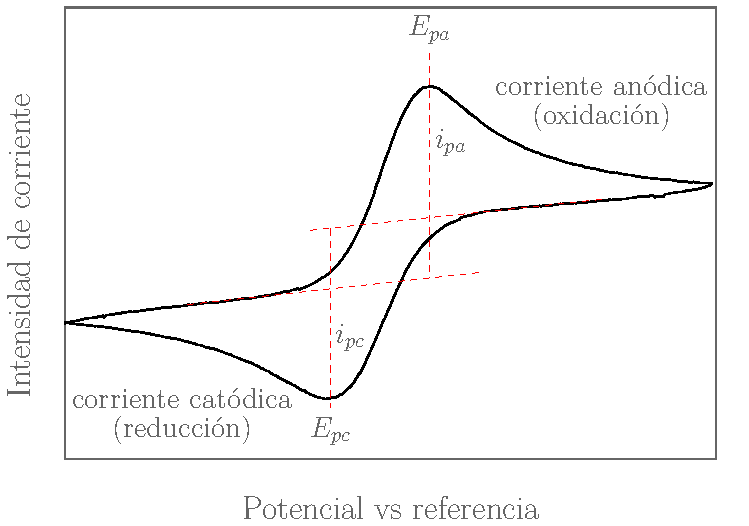
\includegraphics[width=0.65\textwidth]{Esquemas/CV_ideal.pdf}
			 		  \caption[Voltamperograma ideal]{Voltagrama típico para una especie redox reversible.}
			 		  \label{fig:CV_ideal}
			 		  \end{center}
			 		  \end{figure}

	 La voltamperometría cíclica consiste en variar, de una manera cíclica, el potencial de un electrodo estacionario contra un electrodo de referencia\index{electrodo!de referencia}, ambos inmersos en una solución en reposo y medir la corriente resultante. Las señal de excitación es un barrido de potencial lineal con una onda de forma triangular. Las velocidades de barrido pueden variar desde unos cuantos milivolts por segundo hasta cientos de volts por segundo, en nuestro caso se utilizó velocidades próximas a los \SI{50}{\milli\volt.\second^{-1}}. Se barre el potencial del electrodo de trabajo\index{electrodo!de trabajo} en dirección de ida y vuelta entre dos valores arbitrarios. Al\index{aluminio} usar soluciones en base acuosa se debe trabajar en la región de estabilidad electroquímica\index{electroquimico} del H$_2$O, para evitar reducción u oxidación de la misma, que genera H$_2$ u O$_2$ respectivamente. La onda triangular regresa a la misma velocidad y permite la visualización de un voltagrama completo, tal como se muestra en la figura \ref{fig:CV_ideal}, con las formas de las ondas anódicas (oxidación) y catódicas (reducción). 

	 		\begin{figure}[ht!]
			 		  \begin{center}
			 		  \includegraphics[width=\textwidth]{Imagenes/eq.jpg}
			 		  \caption[Equipo para realizar la medidas electroquímica\index{electroquimico}s\index{electroquimico}]{Fotografía del instrumental que se utilizó a lo largo de la Tesis para tomar las medidas electroquímica\index{electroquimico}s\index{electroquimico}.}
			 		  \label{esq:eq}
			 		  \end{center}
			 		  \end{figure}		
	
	 Los parámetros importantes en una voltametría\index{voltametría} cíclico son las magnitudes de la corriente anódica en el pico anódico $i_{pa}$, de la corriente catódica en el pico catódico $i_{pc}$, el potencial del pico catódico $E_{pc}$, el potencial del pico anódico $E_{pa}$, y el área bajo la curva que representa la carga ($Q$) total. 
	 En sistemas idealmente reversibles los picos ánodicos y catódicos son simétricos ($i_{pa}=i_{pc}$) y directamente proporcional a la velocidad de barrido\index{velocidad!de barrido} ($i_p \propto \sqrt{\nu}$); la diferencia de potencial entre ellos es de \SI{59}{\milli\volt} por electrón intercambiado ($E_{pa}-E_{pc}=\SI{59}{\milli\volt\per n}$) e independiente de la velocidad de barrido\index{velocidad!de barrido}. En este tipo de procesos las concentraciones de las distintas especies en la superficie\index{superficie} del electrodo cumplen la ley de Nernst.\cite{Wi2000,Villullas2000,Gosser} Para ello la velocidad de transferencia electrónica\index{transferencia!electrónica}, entre analitos y electrodo, tiene que ser mucho mayor que la velocidad de transferencia de masa, es decir, que la difusión\index{difusión} de las especies hacia el electrodo. Ádemás, si consideramos un electrodo semi-infinito y completamente plano, la corriente de pico para es directamente proporcional a la concentración de la especie que transfiere o toma electrones y, bajo estas condiciones de contorno, la relación queda establecida por la ecuación de Randles-Sevcik\index{Randles-Sevcik}:
				%ecuacion de Randles-sevnic
				\begin{equation}
					i_p=0.4463\: nFAC \left(\frac{nF\upsilon D}{RT}\right)^{\frac{1}{2}}
					\label{eq:randles-sevnic}
				\end{equation}
	 donde 0,446 es el factor para una reacción de transferencia electrónica\index{transferencia!electrónica} simple controlada por difusión\index{difusión}, $n$ es la cantidad de electrones involucrados, $F$ es la constante de Faraday\index{Faraday}, $A$ es el área del electrodo, $C$ la concentración de la especie en solución, $\upsilon$ es la velocidad de barrido\index{velocidad!de barrido}, $D$ el coeficiente de difusión\index{difusión}, $R$ la constante universal de los gases y $T$ la temperatura.

	 Se utilizó una configuración de celda de tres electrodos, electrodo de trabajo\index{electrodo!de trabajo}, contraelectrodo\index{electrodo!contraelectrodo} y referencia. 
	 				\begin{figure}[!ht]
			 		  \begin{center}
			 		  \includegraphics[width=0.75\textwidth]{Esquemas/celda.pdf}
			 		  \caption[Configuración de una celda de tres electrodos]{Configuración de de una celda tres electrodos para realizar medidas electroquímica\index{electroquimico}s\index{electroquimico}.}
			 		  \label{fig:celda}
			 		  \end{center}
			 		  \end{figure}

	 La celda fue fabricada en acrílico y lleva un sello en la parte inferior con un orificio de \SI{1}{\mm} (dando un área geometríca de \SI{3.15}{\mm^{2}}) para sellar contra el sustrato\index{sustrato} y evitar perdidas de la solución, ver la figura \ref{fig:celda}. 
	
	 Las mediciones electroquímica\index{electroquimico}s\index{electroquimico} fueron tomadas con un potencionestato \textit{Teq4}. Como electrodo de referencia\index{electrodo!de referencia} se utilizó un electrodo saturado de calomel (SCE, del ingles \textit{satured calomel electrode}) de la firma \textit{cole-parmer} y como contraelectrodo\index{electrodo!contraelectrodo} se utilizaron indistintamente electrodos de Au\index{electrodo!de Au} depositados por pulverización catódica\index{pulverización catódica} o una pieza de Pt\index{platino}. En la tabla \ref{tabla:eq} se resumen los reactivos utilizados para llevar a cabo las mediciones electroquímica\index{electroquimico}s\index{electroquimico}. 

	 %Esto es porque sino me pone la tabla centrada verticalmente
	 \newpage

	 				%Tabla ractivos EQ
				     \begin{table}[ht!]
			  		  \caption[Reactivos utilizados para las mediciones electroquímica\index{electroquimico}s\index{electroquimico}]{Reactivos utilizados durante las mediciones electroquímica\index{electroquimico}s\index{electroquimico}.}
			  		   \begin{tabular}{>{\raggedright\arraybackslash}m{4.4cm}>{\centering\arraybackslash}m{1.75cm}>{\centering\arraybackslash}m{2.7cm}>{\raggedright\arraybackslash}m{1.6cm}} 
			  		  \toprule
					  Reactivo \hspace{3cm}Nombre& Marca & Peso Molecular (\si{g.mol^{-1}}) & Función  \\ \midrule
			    	  \ferroCompleto \hspace{3cm} ferrocianuro de potasio\index{ferrocianuro de potasio} & \textit{Sigma} & 422,41  & Sonda \\ \midrule
			    	  \ferriCompleto \hspace{3cm} ferrocianuro de potasio\index{ferrocianuro de potasio} & \textit{Sigma} & 329,27  & Sonda  \\ \midrule
			  		  \aminorutenioCompleto  \hspace{3cm}  cloruro de hexaaminorutenio& \textit{Aldrich} &  309,61  & Sonda  \\ \midrule
			  		  \raisebox{-.5\height}{\includegraphics[scale=0.4]{Esquemas/Fc.pdf}}  \hspace{3cm} ferroceno metanol\index{ferroceno metanol}   & \textit{Aldrich} &  216,06 & Sonda  \\ \midrule
			  		  \raisebox{-.5\height}{\includegraphics[scale=0.4]{Esquemas/HQ.pdf}} \hspace{3cm} hidroquinona	& \textit{Biopack} & 110.11  & Sonda  \\ \midrule
			  		  H$_2$O \hspace{3cm} agua &  \SI{18}{\mega\ohm.\cm^{-1}}  &  18,02 & Solvente \\ \midrule
			  		  KCl  \hspace{3cm} cloruro de potasio   & \textit{Biopack} & 74,56 & Electrolito Soporte \\
 			  		  \bottomrule
			    	  \end{tabular}
			   		  \label{tabla:eq}
			   		  \end{table}


% Log del capitulo version final:
% Wanings: 0
% Bad blcks: 11. Todos aceptados:

% B: /home/gustavo/Dropbox/Tesis/Capitulos/materiales.tex:72 Overfull \hbox (17.79167pt too wide) in paragraph ----> Tabla
% B: /home/gustavo/Dropbox/Tesis/Capitulos/materiales.tex:289 Overfull \hbox (5.44995pt too wide) in paragraph ----> Tabla
% B: /home/gustavo/Dropbox/Tesis/Capitulos/materiales.tex:289 Overfull \hbox (2.57881pt too wide) in paragraph ----> Tabla 
% B: /home/gustavo/Dropbox/Tesis/Capitulos/materiales.tex:290 Overfull \hbox (2.40611pt too wide) in paragraph ----> Tabla
% B: /home/gustavo/Dropbox/Tesis/Capitulos/materiales.tex:291 Overfull \hbox (4.66563pt too wide) in paragraph ----> Tabla
% B: /home/gustavo/Dropbox/Tesis/Capitulos/materiales.tex:291 Overfull \hbox (2.40611pt too wide) in paragraph ----> Tabla
% B: /home/gustavo/Dropbox/Tesis/Capitulos/materiales.tex:292 Overfull \hbox (2.40611pt too wide) in paragraph ----> Tabla
% B: /home/gustavo/Dropbox/Tesis/Capitulos/materiales.tex:296 Overfull \hbox (2.40611pt too wide) in paragraph ----> Tabla
% B: /home/gustavo/Dropbox/Tesis/Capitulos/materiales.tex:0 Underfull \vbox (badness 7925) has occurred while \output is active [] -----> Muy apretada una pagina en sentido vertical, Es la imagen de la oblea\index{oblea} V1, sube sobre el encabezado a apenas.
% B: /home/gustavo/Dropbox/Tesis/Capitulos/materiales.tex:0 Underfull \vbox (badness 1406) has occurred while \output is active [] -----> Muy apretada una pagina en sentido vertical, Es la imagen del Sputt, sube apenas sobre el encabezado.
% B: /home/gustavo/Dropbox/Tesis/Capitulos/materiales.tex:536 Overfull \hbox (3.51826pt too wide) in paragraph ----> Tabla


%Agregar proceso de modificacion de la superficie\index{superficie}. Ver Mail de Al\index{aluminio}e W:
%		yo trataría primero la oblea\index{oblea} con el Au\index{oro} depositado. Sobre la superficie\index{superficie} del oro\index{oro} la idea es adsorber el MPTMS desde una solución en algún \%		solvente que esté lo más seco posible (esto para poder reusarla y demorar la hidrólisis/condensación del MPTMS que debería ser poca). %Solventes: tolueno, sería mi primera elección y la concentración 10 mM de MPTMS debería bastar. La adsroción 2 horas es más que suficiente, \%		enjuagar con acetona, secar con N2 o dejar secar y luego al dip coater.